\begin{figure*}[t]
\vspace{-0.7cm}
  \centering
  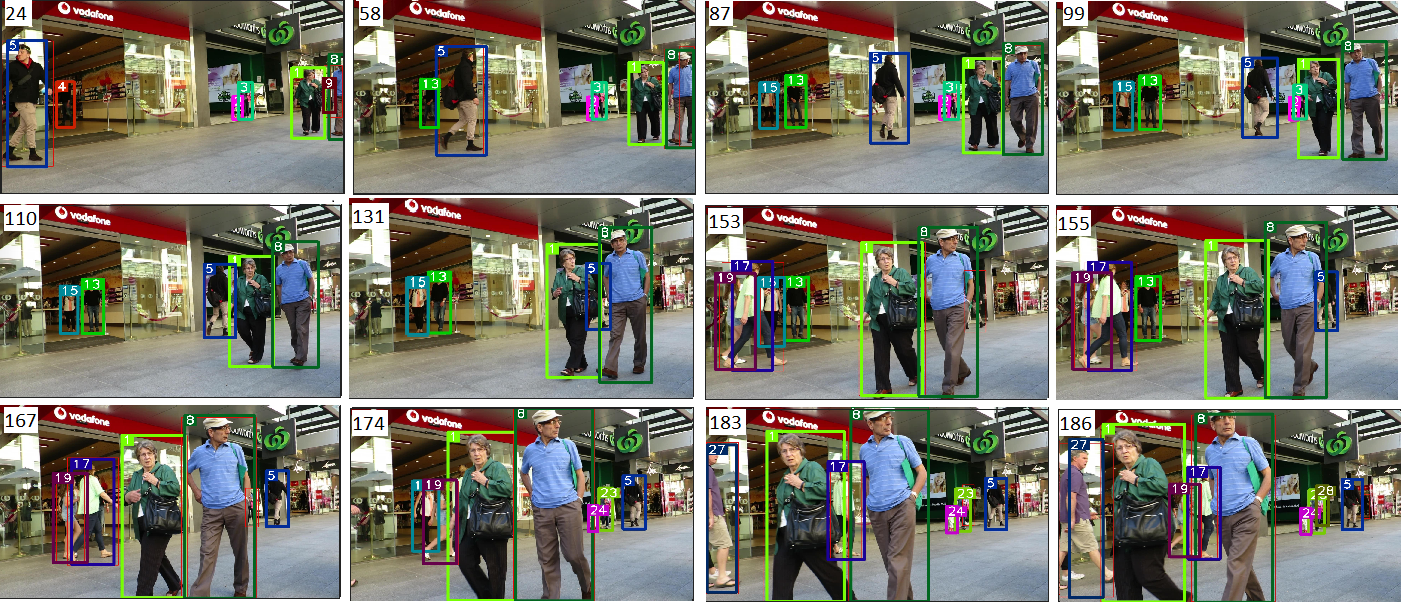
\includegraphics[ width=\textwidth]{figs/occlusions.png}
  \vspace{-0.5cm}
  \caption[Tracking Across Frames]{In the above diagram the numbers on the top left represent the frame number with detection bounding boxes in red and track bounding boxes in other colors. The above diagram depicts the occlusion handling done by our system. It can be seen that track 5(blue) observed in frame 24 is well tracked through out even after been occluded, given that the maximum occlusion duration is less than 30 frames. Additionally tracks 17 and 19 (blue and purple) are reidentified in frame 183 after been occluded. This is because, we control how much the occluding image’s features can affect the track’s template when the track is partially occluded}
  \label{fig:occlusions}
\vspace{1.0cm}
\end{figure*}